\chapter{Inferring empirical ecological networks: everything is biased}\label{appen:Inferring}
In Chapter~\ref{chp:2}, we used empirical ecological networks for our analysis. In the end, the validity of our results will depend on the quality of the data available, and therefore it is important to know some aspects of data collection. \\

The data to recreate an ecological network can be obtained through direct observations (like watching a visit of a certain pollinator to a given flower), indirect observations (like pollen analysis in insects' limbs), or inference (for example based on traits, like the famous Darwin's prediction of the existence of a moth with an enormous proboscis because of the existence of an orchid with extremely long  nectar tubes \cite{darwin1877various}). For the two latter cases, what we are doing is basing the interaction on a proxy. Every method, specifically the second and third one, poses some limitations that could compromise the applicability of our results. Thus, when using empirical networks like in Chapter~\ref{chp:2},  it is convenient to have in mind what are the hidden assumptions in the data collection. \\

We have worked with two different groups of ecological networks. One set has only mutualistic networks from the web service  \href{www.web-of-life.es}{``Web of Life''}. In general, the studies comprise the direct collection of floral and visitor species. A possible limitation of those datasets is the intensity of the survey, together with the presence of any agricultural or other human disruptors that may have stressed the habitat. Fortunately, if we take as a case study our largest dataset \cite{robertson1928flowers}, a second survey at the passage of $75$ years found that more than $82\%$ of the species are still found despite habitat changes \cite{marlin2001native}. \\

\begin{figure}[h!]
     \centering
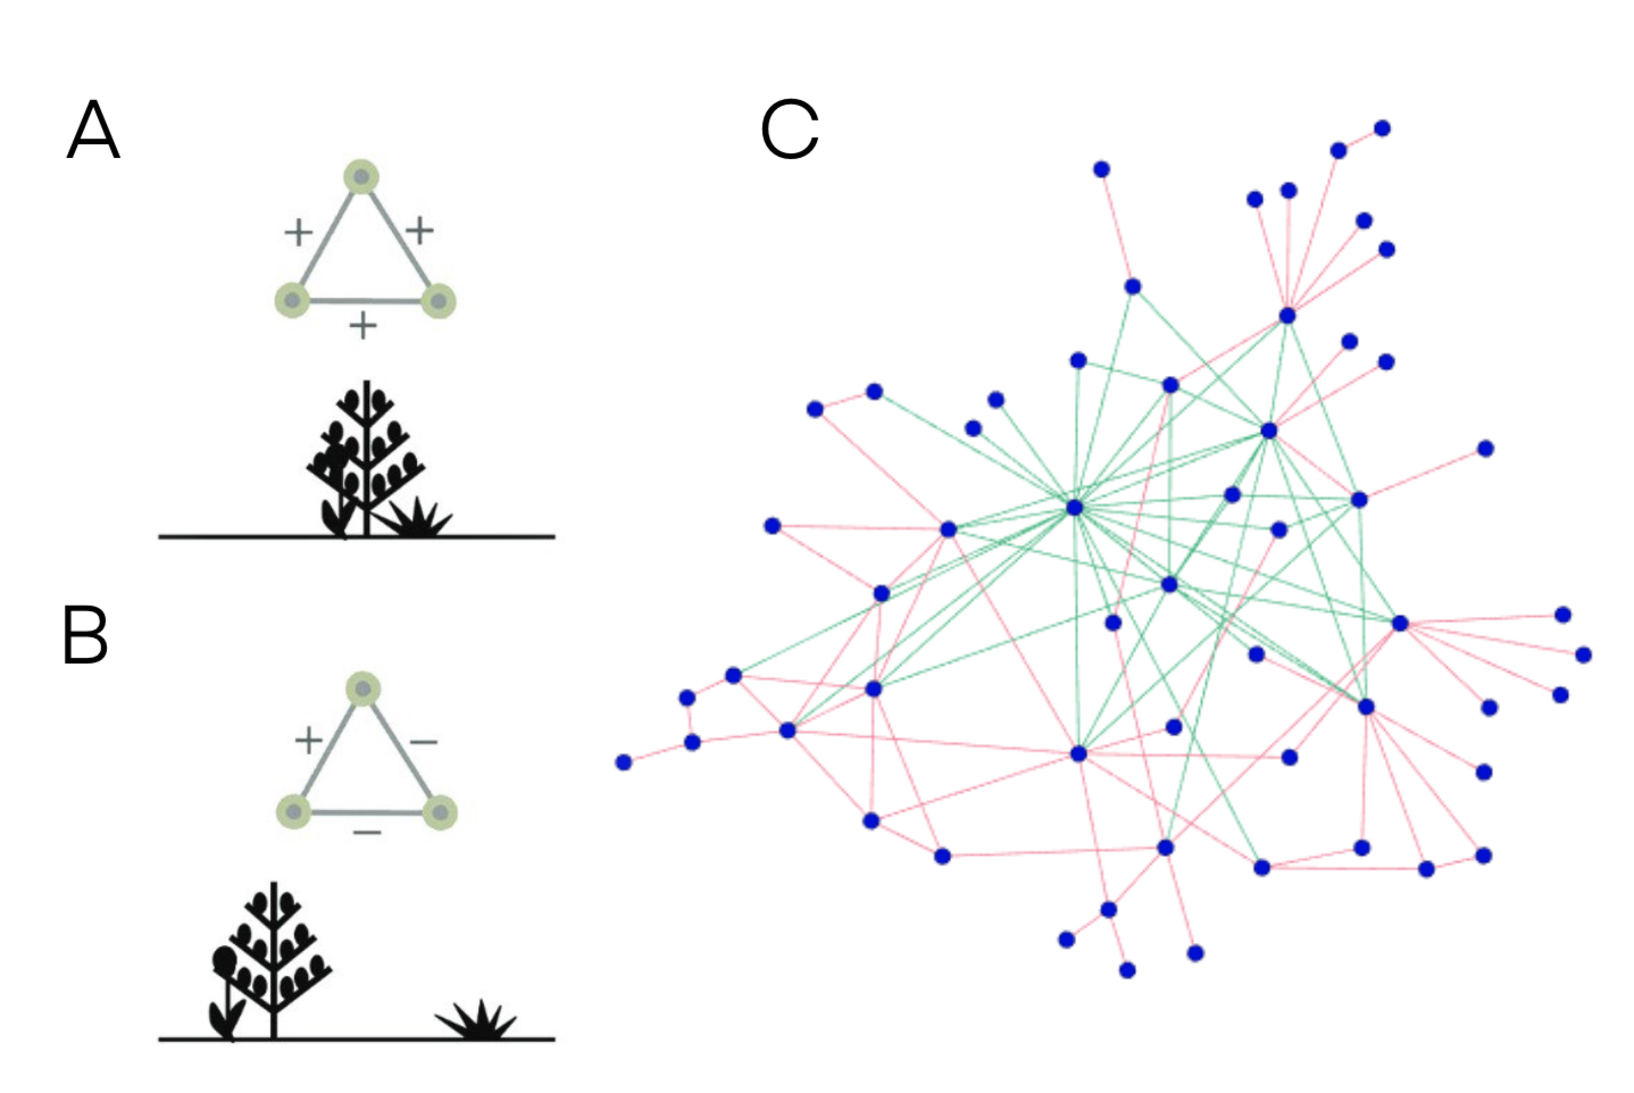
\includegraphics[width=\columnwidth]{figures/methods/fig_hugofacitilation.pdf}
 \caption[Spatial co-occurrence networks]{(Panel a) The ecological interpretation of three spatially associated plants is that of a complete facilitation triad. (Panel b) Two species spatially coexist and the third one segregates for them, hence the negative links. Panels a and b adapted from \cite{Saiz2017EvidenceNetworks}.(Panel c) Visualization of the network $\texttt{Emp}\_\texttt{AE}$ from \cite{Saiz2017EvidenceNetworks}. Each node represents a species and the link color is the type of interaction: green for mutualism and red for competition.}
\label{chp:methods:fig:hugo}
\end{figure}

A more blatant assumption when working with these datasets is the fact that, since they do not record competition, we have supposed competition between guilds is a matter of shared mutualistic patterns. For example, if two pollinators visit the same flowers, they may be competing for the finite amount of nectar. However, in plants, it is not the most crucial competition factor. To overcome this possible limitation, we have also used empirical networks where the spatial distribution of plants determines their competitive interactions \cite{Saiz2017EvidenceNetworks}. Now, the spatial pattern is a proxy for plant competition. A significantly high spatial co-occurrence is a proxy for facilitation or mutualism (Figure~\ref{chp:methods:fig:hugo}a), and significantly low spatial co-occurrence indicates segregation (negative links), which is a proxy for competition in plants communities (Figure~\ref{chp:methods:fig:hugo}b).\\

Local spatial association between pairs of plant species determines the links and their interaction sign in these networks. But abiotic factors can also influence how plants distribute in space. For example, soil composition, sunlight, or underground water sources. Moreover, and in particular, in plant communities, the signs of interactions can change throughout the year \cite{losapio2019perspectives}. However, since the networks are constructed by dominant interactions, these facts should not affect them. Finally, it has been theoretically proven that the relationship between spatial segregation and competition can be reversed if diffusion or continuous niches are considered \cite{hernandez2009species}.  \\

Finally, a common feature of both the visiting and spatial association networks is that they are symmetric and connected. Regarding connectivity, species that are outside the giant component of the interaction network have usually less abundance and dominance, and their effect on the overall is predicted to be almost negligible for our purposes. Symmetry is, per contra, a more delicate issue because it has been recently hypothesized that another alternative key factor for stability in ecosystems could be precisely asymmetry on the interaction strengths \cite{allen2023structural}. 




%%%%%%%%%%%%%%%%%%%%%%%%%%%%%%%%%%%%%%%%%%%%%%%%%%%%%%%%%%%%%%%%%%%%%%%%%%%%%%%%%%%%%%%%%%%%%%%%%%%%%%%
